\documentclass[12pt, letterpaper]{article}
\usepackage{graphicx}
\usepackage{amsmath}
\usepackage{amssymb}
\usepackage{geometry}
\usepackage{array}
\usepackage{xcolor}


\title{Applied Data Science and Artifical Intelligence \\ Assignment 1-a}

\author{Ayush Raina}
\geometry{
  a4paper,
  total={170mm,240mm},
  left=10mm,
  top=10mm,
  right=10mm,
}


\date{\today}
\begin{document}
\maketitle
\large
\section*{Question 1}
We have to test if the mean of hourly bike rentals reduces if "Snowfall" is non zero in winter season. 
\subsection*{Solution}
There are 8760 datapoints in the dataset. We filter out the data points whose "season" is winter. This number is 2160. \textcolor{blue}{There are no non functioning days in winter season.}

\begin{table}[h]
    \centering
    \begin{tabular}{|c|c|c|c|}
    \hline
    season & non-zero Snowfall & zero snowfall & Total \\ \hline
    winter & 392 & 1768 & 2160 \\ \hline
    \end{tabular}
    \caption{Winter Table}
\end{table}

We want to test if the mean of hourly bike rentals reduces if "Snowfall" is non zero in winter season. We will use \textbf{paired t-test} for this. \\

Denote $X_1,X_2,...,X_{392} \sim N(\mu_1,\sigma_1^2)$ and $Y_1,Y_2,...,Y_{1768} \sim N(\mu_2,\sigma_2^2)$ where $X_i$ is the number of bike rentals when snowfall is non-zero and $Y_i$ is the number of bike rentals when snowfall is zero. Here $\mu_1,\mu_2, \sigma_1^2, \sigma_2^2$ all are unknown. \\

We will estimate $\mu_1$ and $\mu_2$ using the sample means $\bar{X}$ and $\bar{Y}$ respectively and $\sigma_1^2$ and $\sigma_2^2$ using the sample variances $S_1^2$ and $S_2^2$ respectively. \\

Define the \textbf{Null Hypothesis:} $H_0: \mu_1 = \mu_2$ ,  \textbf{Alternative Hypothesis:} $H_1: \mu_1 < \mu_2$. \\

Above hypothesis can also be framed as: $H_0: \mu_1 - \mu_2 = 0$ ,  $H_1: \mu_1 - \mu_2 < 0$. \\
Above test can be considered as \textbf{one sided paired t test}. \\

Since $X \sim N(\mu_1,\sigma_1^2)$ and $Y \sim N(\mu_2,\sigma_2^2)$, we can consider $X-Y \sim N(\mu_1-\mu_2,\sigma^2/n + \sigma^2/m)$ where $n=392$ and $m=1768$. We can consider $n \geq 30$ as large enough. Hence we can say that: \\


    \[ \boxed{\frac{\bar{X} - \bar{Y} - (\mu_1 - \mu_2)}{\sqrt{S_1^2/n + S_2^2/m}} \sim N(0,1)} \]

Under the assumption that the null hypothesis is true, $\mu_1 - \mu_2 = 0$. Hence the above equation can be simplified and our Test Statistic becomes: \\

\[ \boxed{T = \frac{\bar{X} - \bar{Y}}{\sqrt{S_1^2/n + S_2^2/m}} } \]

Accept $H_0$ if $T \geq -z_{\alpha}$ \\
Reject $H_0$ if $T < -z_{\alpha}$ \\

On calculating the values we get $\bar{X} = 157.30$, $\bar{Y} = 240.67$, $S_1^2 = 11904.06$, $S_2^2 = 23711.82$. \\

Putting these values in above equation we get $T=-12.599$. \\
Since our signicance level $\alpha = 0.05$, we get $z_{\alpha} = 1.9599$ and clearly we can see that $T < -z_{\alpha}$. Hence we \textbf{reject} the null hypothesis which means that the mean of hourly bike rentals reduces if "Snowfall" is non zero in winter season.

Calculating the p-value for the above test which is equal to $P(Z < -12.599) = 1.05 \times 10^{-36}$ and clearly $\alpha$ is greater than p-value. Hence we reject the null hypothesis.

\section*{Question 2}
Here we have to visualize the hourly non zero rainfall distribution distribution and identify the four quartiles here. Then we have to test if mean count of bike rentals is different in these quartiles using 1 way anova.

\section*{Solution}
There are 8760 datapoints in the dataset out of which 516 data points have non zero rainfall. We can use histogram to visualize the distribution and box plot to identify the quartiles. \\

\textcolor{red}{Non Functioning Days are removed}

\begin{figure}[h]

    \centering
    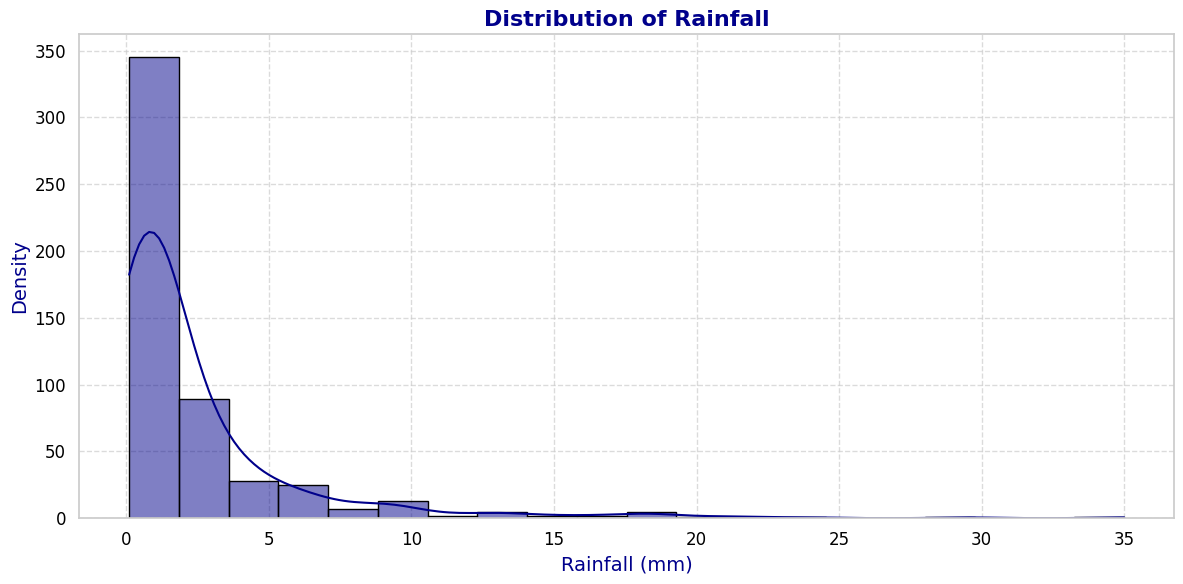
\includegraphics[width=0.9\textwidth]{dist.png}
    \caption{Rainfall Distribution}

    
\end{figure}
Here is the boxplot visualization of the rainfall distribution.
\begin{figure}[h]
    \centering
    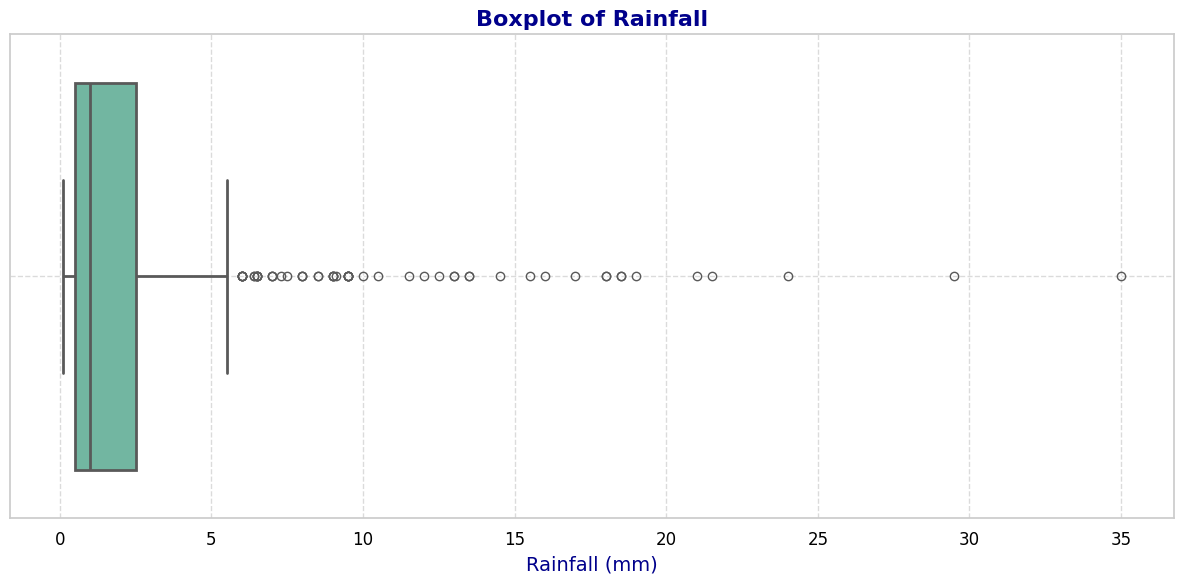
\includegraphics[width=0.9\textwidth]{boxplot2.png}
    \caption{Boxplot of Rainfall Distribution}
\end{figure}

\newpage

\textcolor{blue}{From above boxplot we can clearly see the quartiles and outliers present}

\begin{table}[h]
    \centering
    \begin{tabular}{|c|c|}
    \hline
    count & 516  \\ \hline
    25 \% & 0.5  \\ \hline
    50 \% & 1.0 \\ \hline
    75 \% & 2.5 \\ \hline
    mean & 2.44 \\ \hline
    std deviation & 3.89 \\ \hline
    max & 35 \\ \hline
    \end{tabular}
    \caption{Data distribution}
\end{table}


\newpage 
We now need to test that if the mean count of bike rentals is different in these quartiles using 1 way anova. We will use \textbf{one way anova} for this. \\

\begin{table}[h]
    \centering
    \begin{tabular}{|c|c|}
    \hline
    Quartile & Number of Points  \\ \hline
    1st  & 89  \\ \hline
    2nd  & 121 \\ \hline
    3rd  & 160 \\ \hline
    4th & 146 \\ \hline
    Total & 516 \\ \hline
    \end{tabular}
    \caption{Splitting into Quartiles}
\end{table}

From the below plot, we can visualize hourly bike rentals in these quartiles. \\
\begin{figure}[h]
    \centering
    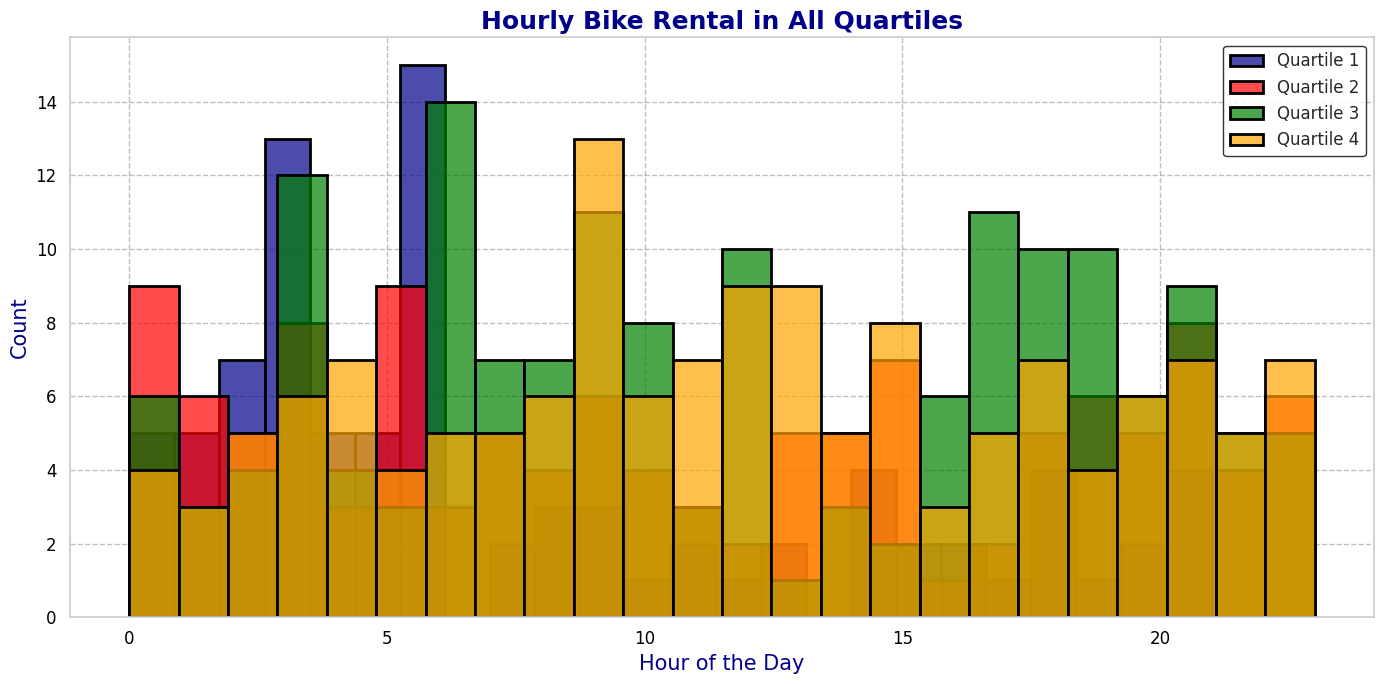
\includegraphics[width=0.7\textwidth]{hourly1.png}
    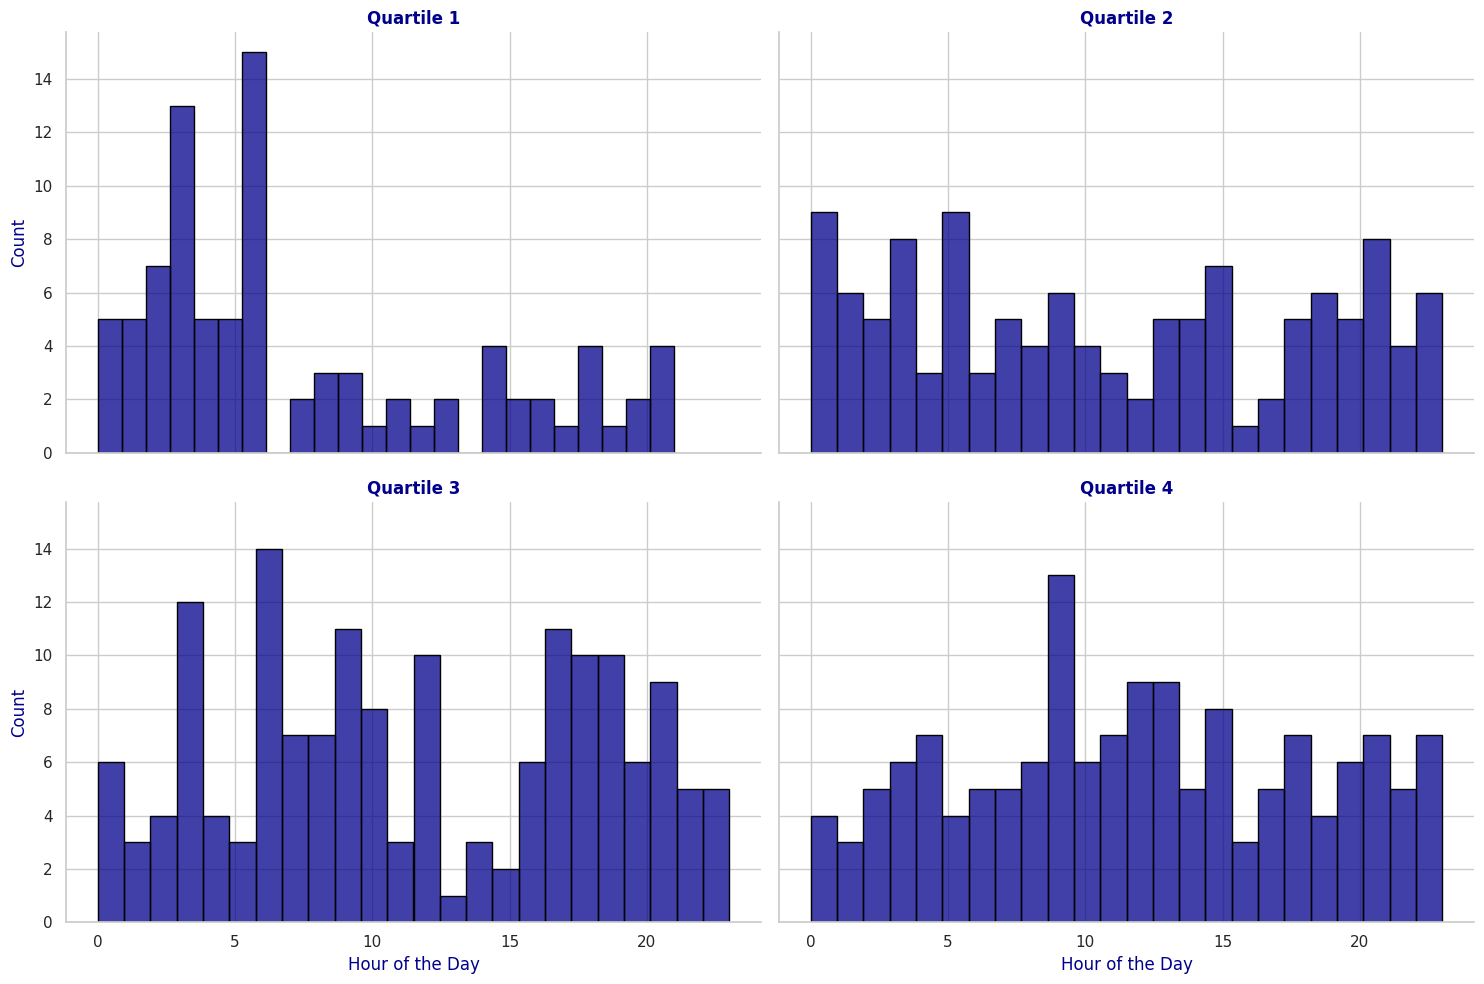
\includegraphics[width=0.7\textwidth]{hourly2.png}
    \caption{Quartiles}
\end{figure}

\newpage

\textcolor{blue}{From above barplots, interesting fact is that there are more bike rentals when there is more rainfall (2nd,4th Quartile) and there are lesser bike rentals in the 1st Quartile.}

\bigskip

Here we have 4 normal samples $X^{(1)},X^{(2)},X^{(3)},X^{(4)}$ of sizes 203,71,118,124 respectively. This is the case of unequal sample sizes.

We can estimate the sample mean of ith population as: 
\[ \boxed{\bar{X^{(i)}} = \frac{1}{n_i} \sum_{j=1}^{n_i} X_j^{(i)}} \]

Then \[Z_{ij} = \frac{X^{(i)}_j-\bar{X^{(i)}}}{\sigma} \sim N(0,1)\] If we take sum of squares of these Z's, we get:

\[ \sum_{i=1}^{4} \sum_{j=1}^{n_i} Z_{ij}^2 \sim \chi^2_{D} \text{ \;\; Chi-Square Random Variable}\]
with $D = \sum_{i=1}^{4} n_i - 4 $ degrees of freedom. \\

\[ \sum_{i=1}^{4} \sum_{j=1}^{n_i} \frac{(X_{ij} - \bar{X^{(i)}})^2}{\sigma^2} \sim \chi^2_{D} \text{ \;\; Chi-Square Random Variable}\]

\[ \text{Let } SS_W = \sum_{i=1}^{4} \sum_{j=1}^{n_i} (X_{ij} - \bar{X^{(i)}})^2 \] 
Then the above equation can be written as:
\[ \frac{SS_W}{\sigma^2} \sim \chi^2_{D}\]

We know that $\mathbb{E}(X) = D$ where $X \sim \chi^2_{D}$. Hence we can write:
\[ \mathbb{E}(\frac{SS_W}{\sigma^2}) = D \]

\[ \implies \boxed{\mathbb{E}(\frac{SS_W}{D})= \sigma^2} \]

It follows that $\frac{SS_W}{D}$ is an unbiased estimator of $\sigma^2$, where $D = \sum_{i=1}^{4} n_i - 4$. \\

We will now find another estimator of $\sigma^2$ which will be a valid estimator when the null hypothesis is true. So let us assume $u_i = \mu$ for all $i$. Then we can write:

\[ \bar{X^{(i)}} \sim N(\mu,\frac{\sigma^2}{n_i}) \]

\[ \sqrt{n_i}\frac{(\bar{X^{(i)}} - \mu)}{\sigma} \sim N(0,1) \]

\[ \sum_{i=1}^{4} \frac{n_i(\bar{X^{(i)}} - \mu)^2}{\sigma^2} \sim \chi^2_{4} \]

We can estimate $\mu$ here by:
\[ \boxed{\bar{\bar{X}} = \frac{1}{4} \sum_{i=1}^{4}  \bar{X^{(i)}}} \] Putting this in above equation we get:

\[ \sum_{i=1}^{4} \frac{n_i(\bar{X^{(i)}} - \bar{\bar{X}})^2}{\sigma^2} \sim \chi^2_{3} \]

\[ \text{Let } SS_B = \sum_{i=1}^{4} n_i(\bar{X^{(i)}} - \bar{\bar{X}})^2 \]

Then it follows when the null hypothesis is true, $\frac{SS_B}{m-1}$ is an unbiased estimator of $\sigma^2$ where $m=4$. \\

Define the Test Statistic as:

\[ \boxed{T= \frac{SS_B/(m-1)}{SS_W/D}} \]

A significant $\alpha$ level test is to :

\[ \text{Reject } H_0 \text{ if } T > F_{m-1,D,\alpha} \]
\[ \text{Accept } H_0 \text{ if } T \leq F_{m-1,D,\alpha} \]

where $D = \sum_{i=1}^{4} n_i - 4$ and $m=4$. \\

In our case $D = 524$, $m=4$, $\bar{X^{(1)}} = 252.05$, $\bar{X^{(2)}} = 252.27$, $\bar{X^{(3)}} = 127.18$, $\bar{X^{(4)}} = 89.02$, $SS_W = 33201816.03$, $SS_B =  2665086.68$, $T = 13.69$, $F_{3,524,0.05} = 2.622$. \\

Since $T > F_{3,524,0.05}$, we reject the null hypothesis. Hence we can say that the mean count of bike rentals is different in these quartiles.

\[ p-value = P(F_{3,524} > 13.69) \]

\[ \boxed{p-value =  1.31e-08} \]


\textcolor{red}{Above results exactly matches with the results obtained from the scipy library and are shown in jupiter notebook.}

\section*{Question 3}
We have to visualize the hourly bike rentals in summer and winter season. Then we have to identify if the two distributions are different using Chi-Square test.

\subsection*{Solution}
Here are the visualizations of the hourly bike rentals in summer and winter season. \\

\textcolor{red}{Non Functioning Days are removed}

\newpage

\textbf{1. Barplots}
\begin{figure}[h]

    \centering
    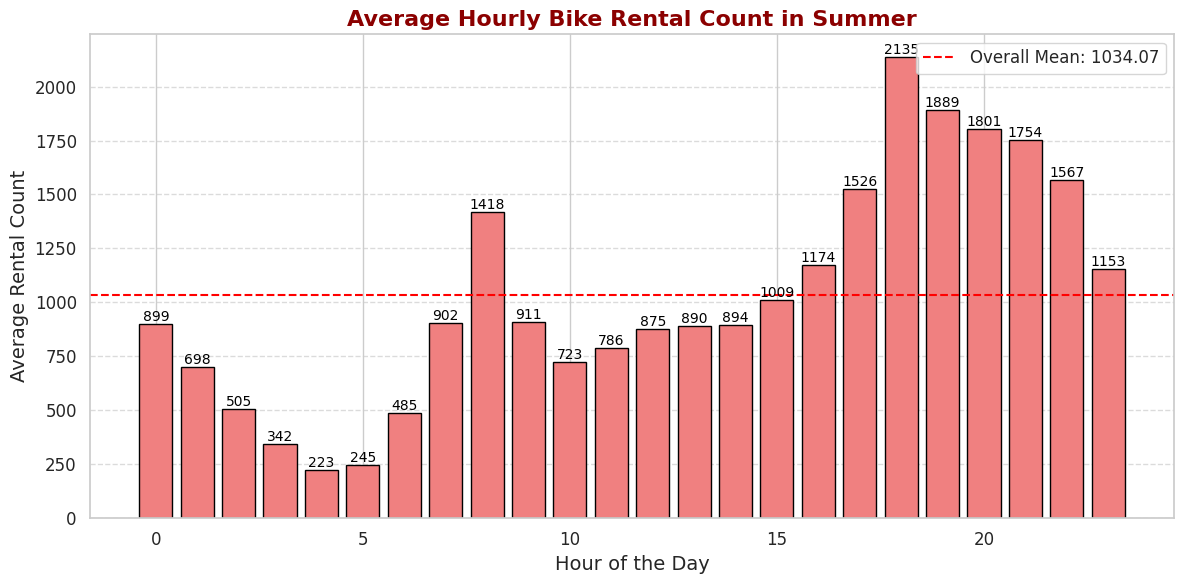
\includegraphics[width=0.8\textwidth]{summer1.png}
    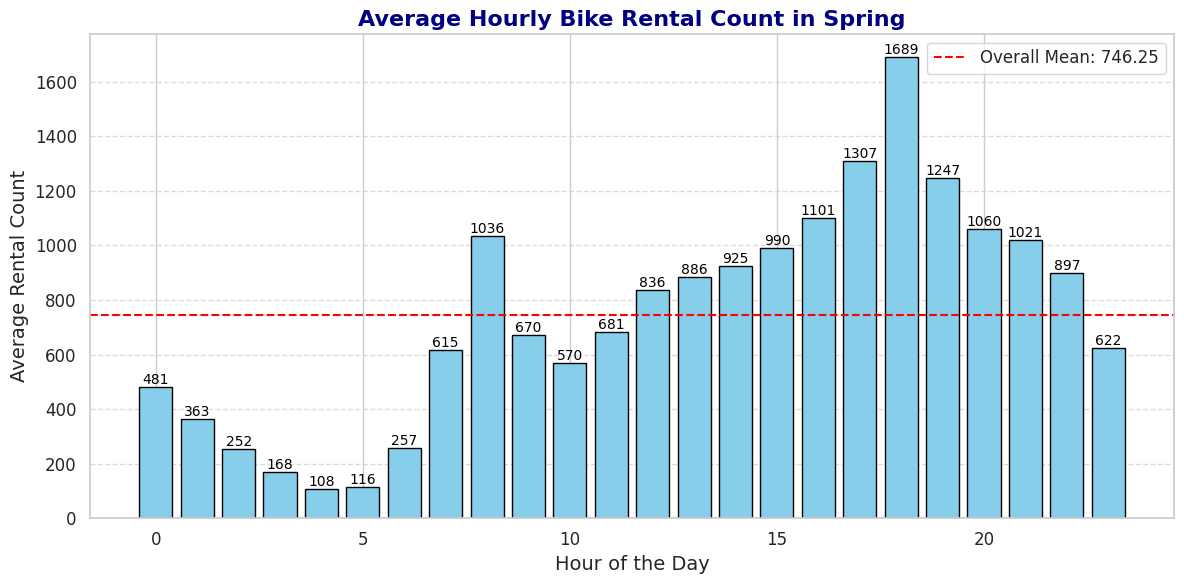
\includegraphics[width=0.8\textwidth]{spring1.png}
    \caption{Summer and Spring Season Rentals}

\end{figure}

\textbf{2. Lineplots and Boxplots}
\begin{figure}[h]

    \centering
    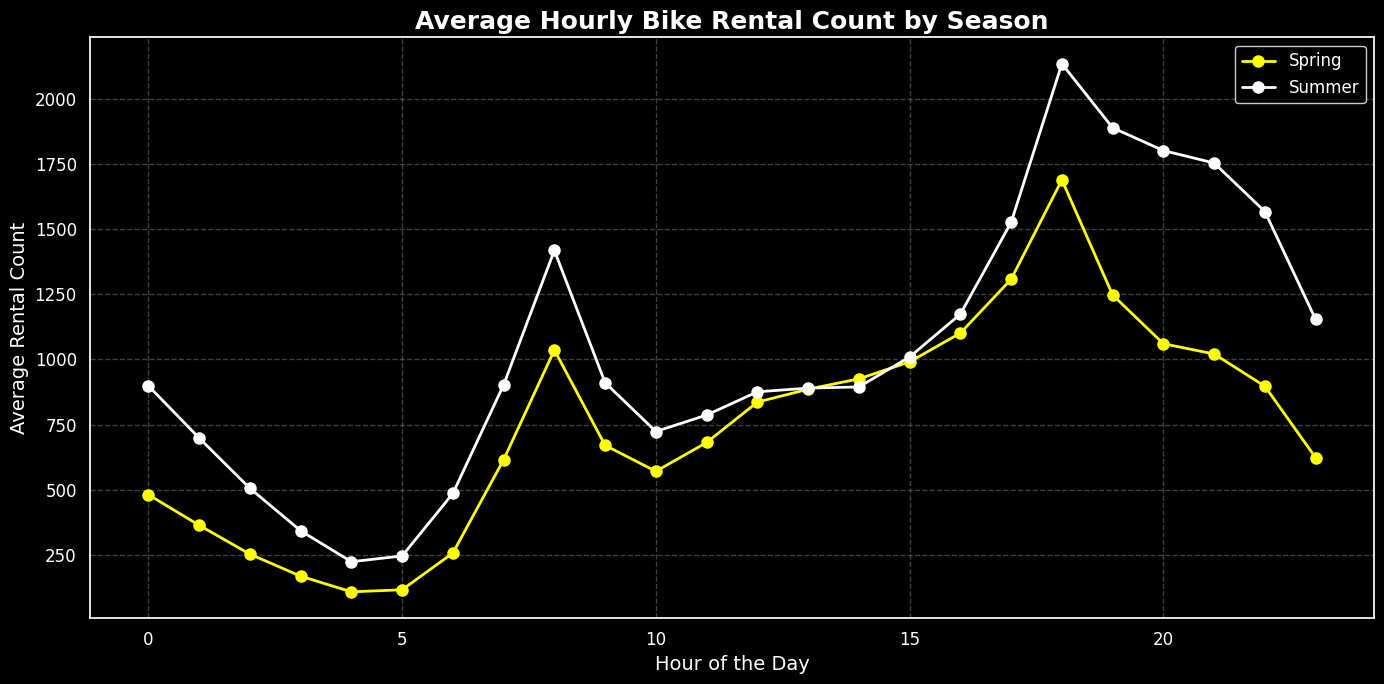
\includegraphics[width=0.8\textwidth]{lineplot1.png}
    \caption{Summer and Spring Season Rentals}

\end{figure}

\begin{figure}[h]

    \centering
    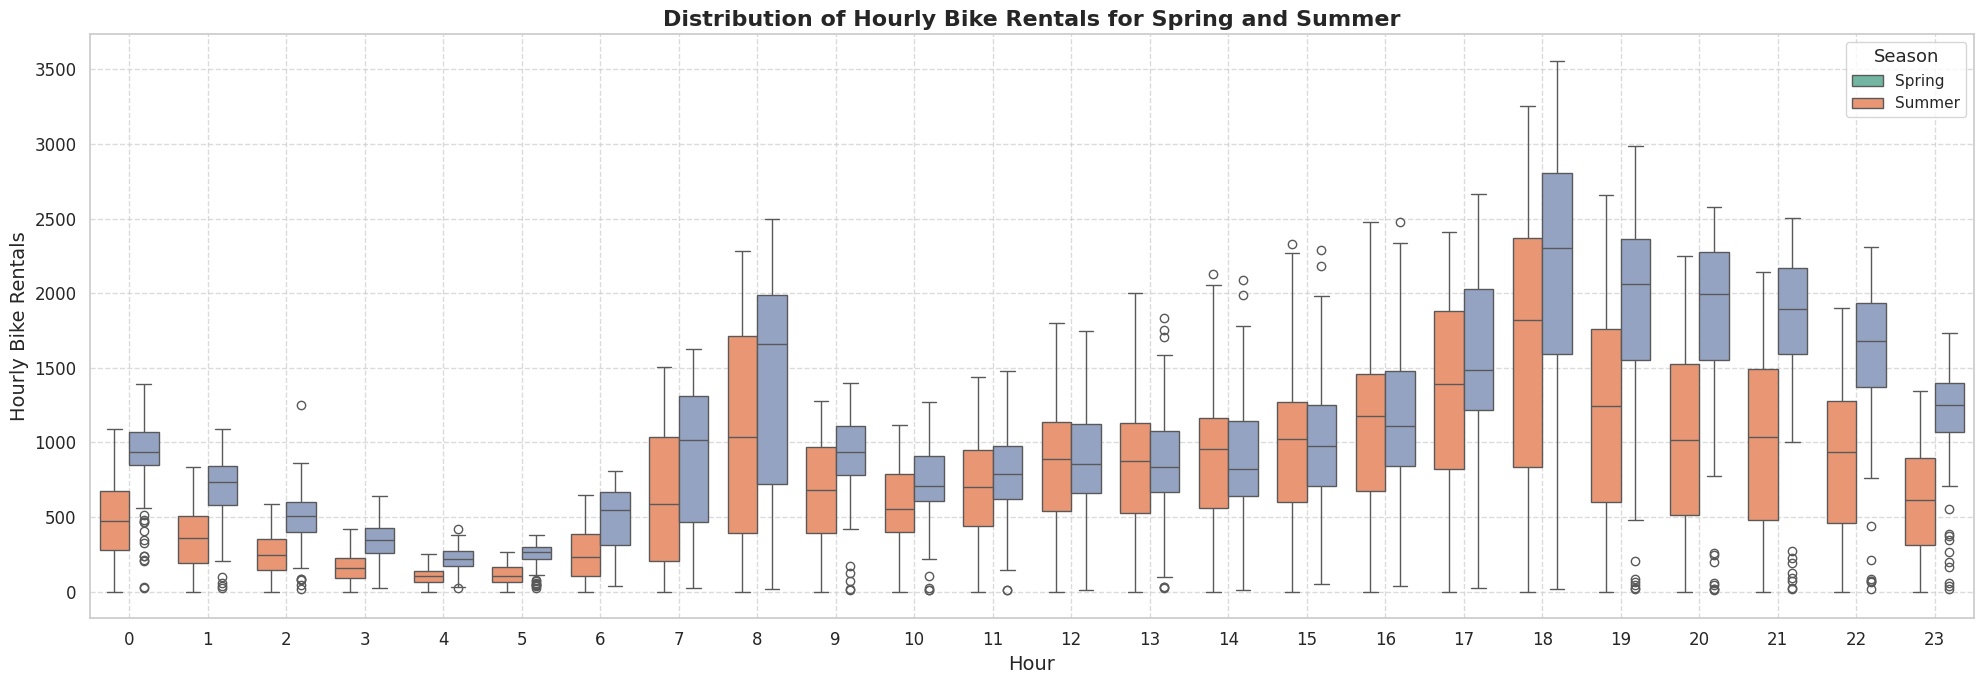
\includegraphics[width=1\textwidth]{boxplot.png}
    \caption{Summer and Spring Season Rentals}

\end{figure}

\newpage
From above box plot we can see that there are many outliers in the data. Before training any ML models we must remove these outliers. \\

Now we have to test if the two distributions are different using Chi-Square test. We will use \textbf{Chi-Square test} for this. \\

\begin{figure}[h]
    \centering
    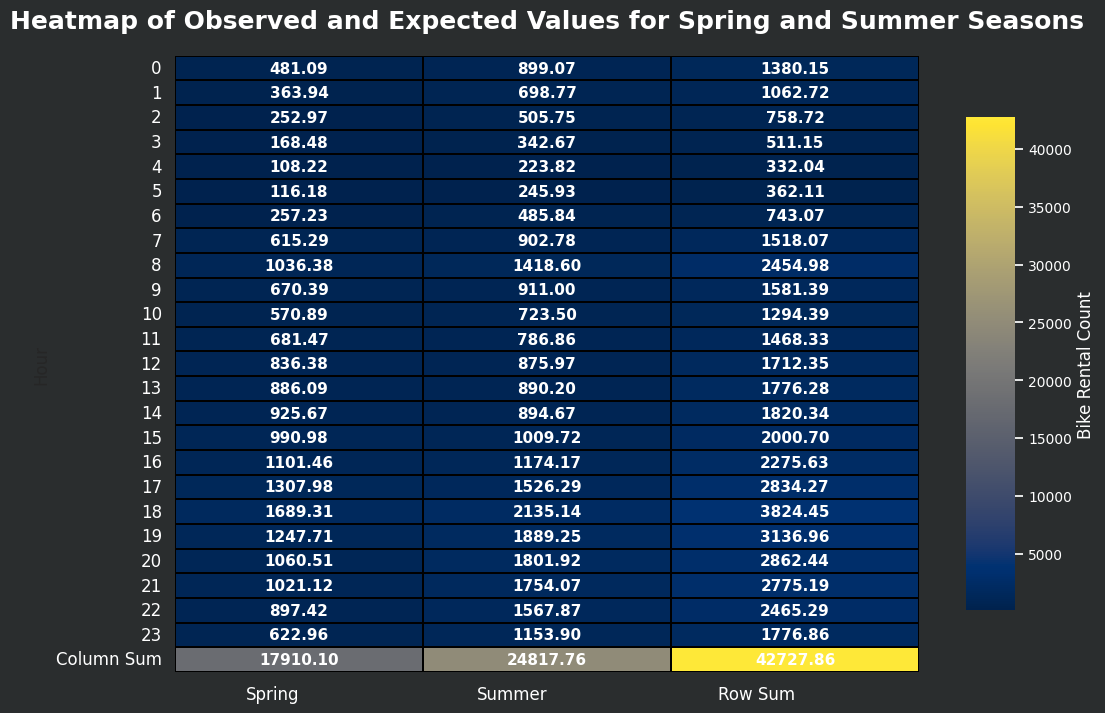
\includegraphics[width=1\textwidth]{heatmap2.png}
    \caption{Chi-Square Test}
\end{figure}

\newpage    

Now we will calculate the Expected Frequency for each cell. We can calculate the Expected Frequency for each cell as:

\[ \boxed{E_{ij} = \frac{\text{row total} \times \text{column total}}{\text{Total Sum}}} \]

where $R_i$ is the sum of the ith row, $C_j$ is the sum of the jth column and $N$ is the total number of observations. \\

Here are the Expected Frequencies for each cell:
\begin{figure}
    \centering
    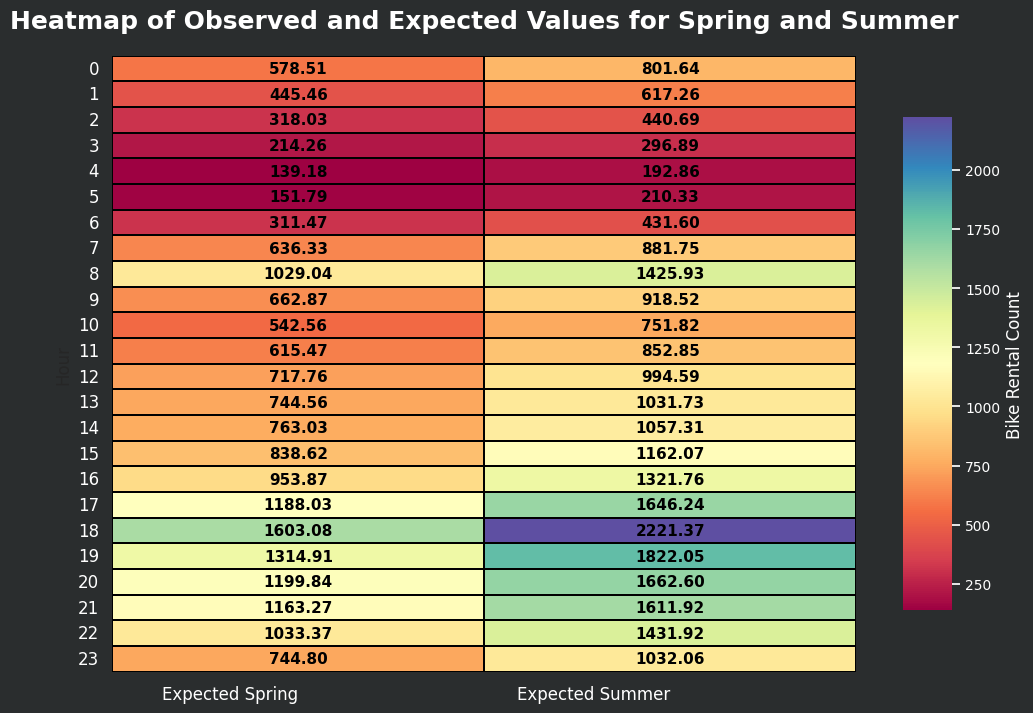
\includegraphics[width=1\textwidth]{heatmap3.png}
    \caption{Expected Frequencies}
\end{figure}

\textcolor{red}{The following values matches with the values obtained from the scipy library.}

\newpage

Now we have expected and observed frequencies for each cell. We can calculate the Chi-Square statistic as: \\

\[ \boxed{T = \sum_{i=1}^{2} \sum_{j=1}^{24} \frac{(O_{ij} - E_{ij})^2}{E_{ij}} } \]

where $O_{ij}$ is the observed frequency and $E_{ij}$ is the expected frequency. \\

On calculating the above equation we get the following results:
\begin{table}[h]
    \centering
    \begin{tabular}{|c|c|}
    \hline
    T &  529.86 \\ \hline
    critical value & 36.41 \\ \hline
    p-value & 1.03e-96 \\ \hline
    \end{tabular}
    \caption{Chi-Square Test Results}
\end{table}

Clearly Test Statistic is greater than critical value, hence we reject the null hypothesis. Hence we can say that the two distributions are different. \\

\textcolor{red}{Above reported values are matching with the values obtained from the scipy library.}

\end{document}
